\documentclass[12pt,a4paper]{article}
\usepackage[utf8]{inputenc}
\usepackage{amsmath}
\usepackage{amsfonts}
\usepackage{amssymb}
\usepackage[none]{hyphenat}
\usepackage{enumerate}
\usepackage[spanish]{babel}
\usepackage{graphicx}
\usepackage{float}
\usepackage{array}
\usepackage{listings}
\usepackage{tcolorbox}
\graphicspath{ {IMAGES/} }
\pagestyle{headings}
\author{Juan Sebastian Gonzalez Camacho (1968220), Andrés Felipe Ruíz Buriticá (1968171), Jhoan Sebastian Rojas Holguin (1958337), Carlos Alberto Delgado Galeano (1968127), Jesus Alberto Gil Ayala (1968231)}
\title{Borvo MO - Requirements Specification}
\begin{document}
\begin{titlepage}
\centering
{\includegraphics[width=0.18 \textwidth]{logo.png} \par}
\vfill
{\bfseries\LARGE Universidad del Valle\par}
{\Large Sede Tuluá\par}
\vfill
{\scshape\Large Ingeniería de Sistemas \par}
\vfill
{\scshape\Huge Borvo - Medicinae Operam \par}
\vfill
{\itshape\Large Avance 1 - Proyecto Final de Bases de Datos y Desarrollo de Software I \par}
\vfill
{\Large Autores: \par}
{\Large Andrés Felipe Ruíz Buriticá - 1968171 \par}
{\Large Carlos Alberto Delgado Galeano - 1968127 \par}
{\Large Jesús Alberto Gil Ayala - 1968231 \par}
{\Large Jhoan Sebastian Rojas Holguin - 1958337 \par}
{\Large Juan Sebastian González Camacho - 1968220 \par}
\vfill
{\Large 8 de Noviembre del 2022 \par}
\end{titlepage}
\tableofcontents
\newpage
\section{Requisitos Específicos}
\subsection{Requerimientos Funcionales}
\newcounter{RF}
\begin{center}
\begin{tabular}{|m{5.5cm}|m{9.5cm}|}
\hline
\textbf{Identificador} & RF-\stepcounter{RF}\arabic{RF}\\
\hline
\textbf{Nombre} & Gestionar afiliados cotizantes de la EPS.\\
\hline
\textbf{Descripción} & El sistema debe permitir gestionar toda la información de los cotizantes de la EPS: Tipo de documento, número de documento de identidad, apellidos, nombres, fecha de nacimiento, género, dirección, ciudad de residencia, teléfono, estado civil, correo electrónico, fecha de la primera afiliación, estado actual (Activo, Inactivo, Retirado), salario, rango salarial. La gestión de esta información está constituida por 4 subrequisitos funcionales:
\begin{itemize}
\item RF-01.1: Registrar cotizante.
\item RF-01.2: Consultar cotizante.
\item RF-01.3: Modificar cotizante.
\item RF-01.4: Eliminar cotizante.
\end{itemize}\\
\hline
\textbf{Prioridad} & Alta.\\
\hline
\end{tabular}
\vspace{5mm}

\begin{tabular}{|m{5.5cm}|m{9.5cm}|}
\hline
\textbf{Identificador} & RF-\stepcounter{RF}\arabic{RF}\\
\hline
\textbf{Nombre} & Gestionar los beneficiarios que tiene cada cotizante.\\
\hline
\textbf{Descripción} & El sistema debe permitir gestionar la información de los  beneficiarios que puede tener cada cotizante: Tipo y número de documento de identidad, apellidos, nombres, fecha de nacimiento, género, dirección, ciudad de residencia, teléfono, estado civil, correo electrónico y parentesco con el cotizante y estado actual. La gestión de esta información está constituida por 4 subrequisitos funcionales:
\begin{itemize}
\item RF-02.1: Registrar beneficiario.
\item RF-02.2: Consultar beneficiario.
\item RF-02.3: Modificar beneficiario.
\item RF-02.4: Eliminar beneficiario.
\end{itemize}\\
\hline
\textbf{Prioridad} & Alta.\\
\hline
\end{tabular}
\vspace{5mm}

\begin{tabular}{|m{5.5cm}|m{9.5cm}|}
\hline
\textbf{Identificador} & RF-\stepcounter{RF}\arabic{RF}\\
\hline
\textbf{Nombre} & Gestionar las empresas que contratan a los cotizantes.\\
\hline
\textbf{Descripción} & El sistema debe permitir gestionar la información de las empresas que contratan a los cotizantes dependientes: Nit, razón social, ciudad, dirección, teléfono, nombre del contacto. En el caso de los trabajadores independientes se debe registrar el mismo cotizante como empresa, registrando el RUT en lugar del Nit y se crea un contrato. La gestión de esta información está constituida en 4 subrequisitos funcionales:
\begin{itemize}
\item RF-03.1: Registrar empresa.
\item RF-03.2: Consultar empresa.
\item RF-03.3: Modificar empresa.
\item RF-03.4: Eliminar empresa.
\end{itemize}\\
\hline
\textbf{Prioridad} & Alta.\\
\hline
\end{tabular}
\vspace{5mm}

\begin{tabular}{|m{5.5cm}|m{9.5cm}|}
\hline
\textbf{Identificador} & RF-\stepcounter{RF}\arabic{RF}\\
\hline
\textbf{Nombre} & Gestionar las IPS que prestan los servicios a sus afiliados.\\
\hline
\textbf{Descripción} & El sistema debe permitir gestionar la información de las IPS que están contratadas por la EPS: Nit, razón social, nivel de atención, servicios que presta. La gestión de esta información está dividida en 4 subrequisitos funcionales:
\begin{itemize}
\item RF-04.1: Registrar IPS.
\item RF-04.2: Consultar IPS.
\item RF-04.3: Modificar IPS.
\item RF-04.4: Eliminar IPS.
\end{itemize}\\
\hline
\textbf{Prioridad} & Alta.\\
\hline
\end{tabular}
\vspace{5mm}

\begin{tabular}{|m{5.5cm}|m{9.5cm}|}
\hline
\textbf{Identificador} & RF-\stepcounter{RF}\arabic{RF}\\
\hline
\textbf{Nombre} & Gestionar órdenes de servicio.\\
\hline
\textbf{Descripción} & El sistema debe permitir gestionar la información de las órdenes de servicio que llevan los afiliados a la EPS, que les entrega la IPS en donde fueron atendidos: Código y fecha de la orden, nombre del médico que la formula, diagnóstico, descripción de los servicios formulados. La gestión de esta información se divide en 2 subrequisitos funcionales:
\begin{itemize}
\item RF-05.1: Registrar órden.
\item RF-05.2: Consultar órden.
\end{itemize}\\
\hline
\textbf{Prioridad} & Alta.\\
\hline
\end{tabular}
\vspace{5mm}

\begin{tabular}{|m{5.5cm}|m{9.5cm}|}
\hline
\textbf{Identificador} & RF-\stepcounter{RF}\arabic{RF}\\
\hline
\textbf{Nombre} & Generar reportes de afiliados.\\
\hline
\textbf{Descripción} & El sistema debe permitir generar los siguientes reportes de los afiliados:
\begin{itemize}
\item RF-06.1: Listado de afiliados por estado.
\item RF-06.2: Listado de afiliados activos de una IPS.
\item RF-06.3: Listado de afiliados inactivos.
\item RF-06.4: Listado de afiliados independientes organizados por estado.
\end{itemize}\\
\hline
\textbf{Prioridad} & Alta.\\
\hline
\end{tabular}
\vspace{5mm}

\begin{tabular}{|m{5.5cm}|m{9.5cm}|}
\hline
\textbf{Identificador} & RF-\stepcounter{RF}\arabic{RF}\\
\hline
\textbf{Nombre} & Generar reportes de órdenes de servicio.\\
\hline
\textbf{Descripción} & El sistema debe permitir generar un reporte de todas las órdenes de servicio por paciente.\\
\hline
\textbf{Prioridad} & Alta.\\
\hline
\end{tabular}
\vspace{5mm}

\begin{tabular}{|m{5.5cm}|m{9.5cm}|}
\hline
\textbf{Identificador} & RF-\stepcounter{RF}\arabic{RF}\\
\hline
\textbf{Nombre} & Reportar pago de aportes.\\
\hline
\textbf{Descripción} & El sistema debe permitir al banco reportar mensualmente el pago de aportes de cada empleado con contrato activo, este reporte debe incluir la fecha de pago, el valor pagado, la información del cotizante y la información de la empresa que hace el pago. Los trabajadores independientes también deben reportar mensualmente su pago de aportes. Este se puede hacer individual o en bloque de archivos.\\
\hline
\textbf{Prioridad} & Alta.\\
\hline
\end{tabular}
\vspace{5mm}

\begin{tabular}{|m{5.5cm}|m{9.5cm}|}
\hline
\textbf{Identificador} & RF-\stepcounter{RF}\arabic{RF}\\
\hline
\textbf{Nombre} & El cotizante puede consultar su propia información.\\
\hline
\textbf{Descripción} & El sistema debe permitir a cada cotizante consultar su propia información.\\
\hline
\textbf{Prioridad} & Media.\\
\hline
\end{tabular}
\vspace{5mm}

\begin{tabular}{|m{5.5cm}|m{9.5cm}|}
\hline
\textbf{Identificador} & RF-\stepcounter{RF}\arabic{RF}\\
\hline
\textbf{Nombre} & Generar listado de pago de aportes.\\
\hline
\textbf{Descripción} & El sistema debe permitir generar un listado de los aportes recibidos por un afiliado en un período de tiempo determinado.\\
\hline
\textbf{Prioridad} & Media.\\
\hline
\end{tabular}
\vspace{5mm}

\begin{tabular}{|m{5.5cm}|m{9.5cm}|}
\hline
\textbf{Identificador} & RF-\stepcounter{RF}\arabic{RF}\\
\hline
\textbf{Nombre} & Generar listado de citas.\\
\hline
\textbf{Descripción} & El sistema debe permitir generar un listado de citas en una fecha e IPS en particular.\\
\hline
\textbf{Prioridad} & Media.\\
\hline
\end{tabular}
\vspace{5mm}
\end{center}
\subsection{Requerimientos No Funcionales}
\newcounter{RNF}
\begin{center}
\begin{tabular}{|m{5.5cm}|m{9.5cm}|}
\hline
\textbf{Identificador} & RNF-\stepcounter{RNF}\arabic{RNF}\\
\hline
\textbf{Nombre} & Diseño de interfaz amigable.\\
\hline
\textbf{Descripción} & El software debe ser sencillo e intuitivo para una mejor comprensión de los usuarios.\\
\hline
\textbf{Categoría} & Usabilidad.\\
\hline
\end{tabular}
\vspace{5mm}

\begin{tabular}{|m{5.5cm}|m{9.5cm}|}
\hline
\textbf{Identificador} & RNF-\stepcounter{RNF}\arabic{RNF}\\
\hline
\textbf{Nombre} & Software ágil.\\
\hline
\textbf{Descripción} & El software debe generar la información y mostrar formularios y guías claros y concisos.\\
\hline
\textbf{Categoría} & Usabilidad.\\
\hline
\end{tabular}
\vspace{5mm}

\begin{tabular}{|m{5.5cm}|m{9.5cm}|}
\hline
\textbf{Identificador} & RNF-\stepcounter{RNF}\arabic{RNF}\\
\hline
\textbf{Nombre} & Disponible.\\
\hline
\textbf{Descripción} & El software estará en funcionamiento todo el tiempo.\\
\hline
\textbf{Categoría} & Desempeño.\\
\hline
\end{tabular}
\vspace{5mm}

\begin{tabular}{|m{5.5cm}|m{9.5cm}|}
\hline
\textbf{Identificador} & RNF-\stepcounter{RNF}\arabic{RNF}\\
\hline
\textbf{Nombre} & Tolerante al error.\\
\hline
\textbf{Descripción} & El sistema proveerá información con respecto al error en la ejecución de alguna función y añadirá una recomendación.\\
\hline
\textbf{Categoría} & Desempeño.\\
\hline
\end{tabular}
\vspace{5mm}

\begin{tabular}{|m{5.5cm}|m{9.5cm}|}
\hline
\textbf{Identificador} & RNF-\stepcounter{RNF}\arabic{RNF}\\
\hline
\textbf{Nombre} & Permisos de usuario.\\
\hline
\textbf{Descripción} & El sistema solicitará usuario y contraseña para determinar los permisos según el perfil de usuario.\\
\hline
\textbf{Categoría} & Seguridad.\\
\hline
\end{tabular}
\vspace{5mm}

\begin{tabular}{|m{5.5cm}|m{9.5cm}|}
\hline
\textbf{Identificador} & RNF-\stepcounter{RNF}\arabic{RNF}\\
\hline
\textbf{Nombre} & Personal autorizado.\\
\hline
\textbf{Descripción} & Al sistema solo pueden ingresar los usuarios autorizados que están registrados en la base de datos.\\
\hline
\textbf{Categoría} & Seguridad.\\
\hline
\end{tabular}
\vspace{5mm}

\begin{tabular}{|m{5.5cm}|m{9.5cm}|}
\hline
\textbf{Identificador} & RNF-\stepcounter{RNF}\arabic{RNF}\\
\hline
\textbf{Nombre} & Tiempo de respuesta\\
\hline
\textbf{Descripción} & El sistema debe enviar una respuesta en el acceso y uso de sus funciones en no más de 10 segundos.\\
\hline
\textbf{Categoría} & Eficiencia.\\
\hline
\end{tabular}
\vspace{5mm}

\begin{tabular}{|m{5.5cm}|m{9.5cm}|}
\hline
\textbf{Identificador} & RNF-\stepcounter{RNF}\arabic{RNF}\\
\hline
\textbf{Nombre} & Acceso desde varios dispositivos.\\
\hline
\textbf{Descripción} & El sistema debe ser un aplicativo web que permita ingresar desde cualquier dispositivo.\\
\hline
\textbf{Categoría} & Portabilidad.\\
\hline
\end{tabular}
\vspace{5mm}
\end{center}
\subsection{Diagrama de Casos de Uso}
\begin{figure}[H]
\centering
{\includegraphics[width=1 \textwidth]{use_cases_diagram.pdf} \par}
\caption{Diagrama de Casos de Uso.}
\end{figure}
\subsection{Especificación de Casos de Uso}
\newcounter{CU}
\begin{center}
\begin{tabular}{|m{5.5cm}| m{9.5cm}|}
\hline 
\multicolumn{2}{|c|}{\textbf{CU-\stepcounter{CU}\arabic{CU} GestionarAfiliado}} \\ 
\hline 
\textbf{Descripción} & Permite registrar la información de los afiliados. \\ 
\hline 
\textbf{Actores} & Es iniciado por Administrador. \\ 
\hline 
\textbf{Pre-condición} & El administrador debe estar dentro del sistema. \\ 
\hline 
\textbf{Flujo de Eventos} & Flujo Principal (P):

\textbf{P1.} El administrador debe seleccionar la opción Gestionar afiliado en el sistema.

\textbf{P2.} El sistema despliega un formulario para registrar los datos de los afiliados.

\textbf{P3.} El administrador registra DNI, Nombres, Apellidos, Fecha de Nacimiento, Ciudad de Residencia, Teléfono, e-mail, Dirección, Género, Estado Civil, Estado Actual, Fecha de Primera Afiliación, Salario, Rango Salarial.

\textbf{P4.} Si el afiliado tiene beneficiarios se inicia el \emph{CU GestionarBeneficiario} para su respectivo registro.

\textbf{P5.} El administrador da clic en el botón Guardar para enviar el formulario.

\textbf{P6.} El sistema valida los datos (A1).

\textbf{P7.} El sistema muestra el mensaje de confirmación.
\\
\hline 
\textbf{Flujo Alterno} &  Flujo Alterno (A):

\textbf{A1.} El afiliado ya se encontraba registrado.

	En P6:
	
	6.1. Si el DNI corresponde a un afiliado ya registrado, el sistema debe mostrar un mensaje indicando esto.
	
	6.2. Si es error de digitación, retorna a P2 para ingresar nuevamente los datos en el formulario. \\ 
\hline 
\textbf{Post-condición}  & El afiliado queda registrado en el sistema. \\ 
\hline 
\textbf{Requisitos No Funcionales} & Ninguno \\ 
\hline 
\end{tabular}
\vspace{5mm}

\begin{tabular}{|m{5.5cm}| m{9.5cm}|}
\hline 
\multicolumn{2}{|c|}{\textbf{CU-\stepcounter{CU}\arabic{CU} GestionarContratosIPS}} \\ 
\hline 
\textbf{Descripción} & Permite registrar una IPS dentro del sistema. \\ 
\hline 
\textbf{Actores} & Es iniciado por Administrador.\\ 
\hline 
\textbf{Pre-condición} & El administrador ¿debe estar dentro del sistema.\\ 
\hline 
\textbf{Flujo de Eventos} & Flujo Principal (P):

\textbf{P1.} El administrador selecciona la opción de Registrar nueva IPS.

\textbf{P2.} El sistema despliega un formulario para registrar la IPS.

\textbf{P3.} El administrador ingresa el NIT, razón social, nivel de atención y servicios que presta la IPS.

\textbf{P4.} El administrador da clic en el botón Guardar para enviar el formulario.

\textbf{P5.} El sistema valida los datos (A1).

\textbf{P6.} El sistema muestra el mensaje de confirmación.
\\
\hline 
\textbf{Flujo Alterno} &  Flujo Alterno (A):

\textbf{A1.} La IPS ya está registrada.

	En P5:
	
	5.1. Si el NIT corresponde a una IPS ya registrada, el sistema debe mostrar un mensaje indicando esto.
	
	5.2. Si es error de digitación, retorna a P2 para ingresar nuevamente los dato sen el formulario. \\ 
\hline 
\textbf{Post-condición}  & Registro exitoso de la IPS dentro del sistema. \\ 
\hline 
\textbf{Requisitos No Funcionales} & Ninguno \\ 
\hline 
\end{tabular}
\vspace{5mm}

\begin{tabular}{|m{5.5cm}| m{9.5cm}|}
\hline 
\multicolumn{2}{|c|}{\textbf{CU-\stepcounter{CU}\arabic{CU} GestionarOrdenDeServicio}} \\ 
\hline 
\textbf{Descripción} & Permite registrar las ordenes de servicio que llevan los afiliados, expedidas por las IPS. \\ 
\hline 
\textbf{Actores} & Es iniciado por Administrador.\\ 
\hline 
\textbf{Pre-condición} & El administrador ¿debe estar dentro del sistema.\\ 
\hline 
\textbf{Flujo de Eventos} & Flujo Principal (P):

\textbf{P1.} El administrador selecciona la opción de Registrar nueva Orden de Servicio.

\textbf{P2.} El sistema despliega un formulario para registrar la orden de servicio.

\textbf{P3.} El administrador ingresa el Código, fecha de la orden, nombre del médico que formula, diagnóstico, descripción de los servicios formulados.

\textbf{P4.} El administrador da clic en el botón Guardar para enviar el formulario.

\textbf{P5.} El sistema valida los datos (A1).

\textbf{P6.} El sistema muestra el mensaje de confirmación.
\\
\hline 
\textbf{Flujo Alterno} &  Flujo Alterno (A):

\textbf{A1.} La orden de servicio ya está registrada.

	En P5:
	
	5.1. Si el código corresponde a una orden ya registrada, el sistema debe mostrar un mensaje indicando esto.
	
	5.2. Si es error de digitación, retorna a P2 para ingresar nuevamente los dato sen el formulario. \\ 
\hline 
\textbf{Post-condición}  & Registro exitoso de la orden de servicio dentro del sistema. \\ 
\hline 
\textbf{Requisitos No Funcionales} & Ninguno \\ 
\hline 
\end{tabular}
\vspace{5mm}

\begin{tabular}{|m{5.5cm}| m{9.5cm}|}
\hline 
\multicolumn{2}{|c|}{\textbf{CU-\stepcounter{CU}\arabic{CU} GestionarEmpresa}} \\ 
\hline 
\textbf{Descripción} & Permite registrar la información de las empresas a las que pertenecen los afiliados. \\ 
\hline 
\textbf{Actores} & Es iniciado por Administrador. \\ 
\hline 
\textbf{Pre-condición} & El administrador debe haberse autenticado de forma exitosa en el sistema de acuerdo a su perfil. \\ 
\hline 
\textbf{Flujo de Eventos} & Flujo Principal (P):

\textbf{P1.} El administrador debe seleccionar la opción Gestionar empresa en el sistema.

\textbf{P2.} El sistema despliega un formulario para registrar los datos de las empresas.

\textbf{P3.} El administrador registra NIT, Ciudad, Teléfono, Razón social, Nombre del contacto.

\textbf{P4.} El administrador da clic en el botón Guardar para enviar el formulario.

\textbf{P5.} El sistema valida los datos (A1).

\textbf{P6.} El sistema muestra el mensaje de confirmación.
\\
\hline 
\textbf{Flujo Alterno} &  Flujo Alterno (A):

\textbf{A1.} La empresa ya se encontraba registrada.

	En P5:
	
	5.1. Si el NIT corresponde a una empresa ya registrada, el sistema debe mostrar un mensaje indicando esto.
	
	5.2. Si es error de digitación, retorna a P2 para ingresar nuevamente los datos en el formulario. \\ 
\hline 
\textbf{Post-condición}  & La empresa queda registrada en el sistema. \\ 
\hline 
\textbf{Requisitos No Funcionales} & Ninguno \\ 
\hline 
\end{tabular}
\vspace{5mm}

\begin{tabular}{|m{5.5cm}| m{9.5cm}|}
\hline 
\multicolumn{2}{|c|}{\textbf{CU-\stepcounter{CU}\arabic{CU} GenerarReportes}} \\ 
\hline 
\textbf{Descripción} & Permite generar reportes. \\ 
\hline 
\textbf{Actores} & Es iniciado por Administrador. \\ 
\hline 
\textbf{Pre-condición} & El administrador debe estar dentro del sistema. \\ 
\hline 
\textbf{Flujo de Eventos} & Flujo Principal (P):

\textbf{P1.} El administrador selecciona la opción de generar reportes.

\textbf{P2.} El sistema despliega los tipos de reporte que se pueden realizar.

\textbf{P3.} El administrador selecciona el tipo de reporte que desea (A1).

\textbf{P4.} El sistema muestra un mensaje de confirmación.
\\
\hline 
\textbf{Flujo Alterno} &  Flujo Alterno (A):

\textbf{A1.}Selección del tipo de reporte.

	En P3:
	
	3.1. Si el tipo de reporte es Afiliados por Estado, se ejecutará el caso de uso \emph{AfiliadosPorEstado}.
	
	3.2. Si el tipo de reporte es Órdenes por Paciente, se ejecutará el caso de uso \emph{ÓrdenesPorPaciente}.
	
	3.3. Si el tipo de reporte es Afiliados por Empresa, se ejecutará el caso de uso \emph{AfiliadosPorEmpresa}.\\ 
\hline 
\textbf{Post-condición}  & Generación de cualquier tipo de reporte. \\ 
\hline 
\textbf{Requisitos No Funcionales} & Ninguno \\ 
\hline 
\end{tabular}
\vspace{5mm}

\begin{tabular}{|m{5.5cm}| m{9.5cm}|}
\hline 
\multicolumn{2}{|c|}{\textbf{CU-\stepcounter{CU}\arabic{CU} ConsultarAfiliación}} \\ 
\hline 
\textbf{Descripción} & Permite consultar la información del cotizante actualmente autenticado. \\ 
\hline 
\textbf{Actores} & Es iniciado por Cotizante. \\ 
\hline 
\textbf{Pre-condición} & El cotizante debe haberse autenticado de forma exitosa en el sistema de acuerdo a su usuario y contraseña en el caso de uso \emph{IniciarSesión}. \\ 
\hline 
\textbf{Flujo de Eventos} & Flujo Principal (P):

\textbf{P1.} El cotizante selecciona la opción de Consultar Información.

\textbf{P2.} El sistema despliega una página con la información del cotizante y sus beneficiarios (si los tiene).
\\
\hline 
\textbf{Flujo Alterno} &  Flujo Alterno (A):
\\ 
\hline 
\textbf{Post-condición}  & El cotizante consulta su propia información que está guardada en el sistema. \\ 
\hline 
\textbf{Requisitos No Funcionales} & Ninguno \\ 
\hline 
\end{tabular}
\vspace{5mm}

\begin{tabular}{|m{5.5cm}| m{9.5cm}|}
\hline 
\multicolumn{2}{|c|}{\textbf{CU-\stepcounter{CU}\arabic{CU} ReportarPagoAportes}} \\ 
\hline 
\textbf{Descripción} & Permite reportar dentro del sistema el pago de aportes que hace cada cotizante. \\ 
\hline 
\textbf{Actores} & Es iniciado por Banco. \\ 
\hline 
\textbf{Pre-condición} & El banco debe estar dentro del sistema. \\ 
\hline 
\textbf{Flujo de Eventos} & Flujo Principal (P):

\textbf{P1.} El banco selecciona la opción de Reporte pago de aportes.

\textbf{P2.} El sistema despliega los tipos de reporte que se pueden hacer.

\textbf{P3.} El banco selecciona el tipo de reporte que desea realizar. (A1)

\textbf{P4.} El banco da clic en el botón Guardar para enviar el formulario.

\textbf{P5.} El sistema valida los datos (A2).

\textbf{P6.} El sistema muestra un mensaje de confirmación.
\\
\hline 
\textbf{Flujo Alterno} &  Flujo Alterno (A):

\textbf{A1.} Seleccionar el tipo de reporte a realizar.

	En P3:
	
	3.1. Si el tipo de reporte es individual, se ejecutará el caso de uso \emph{ReporteIndividual}.
	
	3.2. Si el tipo de reporte es en bloque, se ejecutará el caso de uso \emph{ReporteBloque}.
	
\textbf{A2.} El pago de aportes ya se ha realizado.

	En P5:
	
	5.1. Si no hay un pago de aportes pendiente, el sistema debe mostrar un mensaje indicando esto.
	
	5.2. Si es error de digitación, retorna a P2 para ingresar nuevamente los dato sen el formulario. \\ 
\hline 
\textbf{Post-condición}  & Reporte de pago de aportes realizados durante el mes. \\ 
\hline 
\textbf{Requisitos No Funcionales} & Ninguno \\ 
\hline 
\end{tabular}
\vspace{5mm}

\begin{tabular}{|m{5.5cm}| m{9.5cm}|}
\hline 
\multicolumn{2}{|c|}{\textbf{CU-\stepcounter{CU}\arabic{CU} ReportarNovedad}} \\ 
\hline 
\textbf{Descripción} & Permite reportar una novedad, ya sea una vinculación o un retiro de la de un cotizante en alguna empresa. \\ 
\hline 
\textbf{Actores} & Es iniciado por Banco. \\ 
\hline 
\textbf{Pre-condición} & El banco debe estar dentro del sistema. \\ 
\hline 
\textbf{Flujo de Eventos} & Flujo Principal (P):

\textbf{P1.} El banco selecciona la opción de Reportar Novedad.

\textbf{P2.} El sistema despliega los tipos de reporte que se pueden hacer.

\textbf{P3.} El banco selecciona el tipo de reporte que desea realizar. (A1)
\\
\hline 
\textbf{Flujo Alterno} &  Flujo Alterno (A):

\textbf{A1.} Seleccionar el tipo de reporte a realizar.

	En P3:
	
	3.1. Si el tipo de reporte es vinculación, se ejecutará el caso de uso \emph{ReportarVinculación}.
	
	3.2. Si el tipo de reporte es en retiro, se ejecutará el caso de uso \emph{ReportarRetiro}\\ 
\hline 
\textbf{Post-condición}  & Reporte de novedad realizado correctamente. \\ 
\hline 
\textbf{Requisitos No Funcionales} & Ninguno \\ 
\hline 
\end{tabular}
\vspace{5mm}

\begin{tabular}{|m{5.5cm}| m{9.5cm}|}
\hline 
\multicolumn{2}{|c|}{\textbf{CU-\stepcounter{CU}\arabic{CU} IniciarSesión}} \\ 
\hline 
\textbf{Descripción} & Permite al usuario ingresar al sistema según su rol. \\ 
\hline 
\textbf{Actores} & Es iniciado por Administrador, Cotizante o Banco. \\ 
\hline 
\textbf{Pre-condición} & El usuario debe estar previamente registrado en el sistema. \\ 
\hline 
\textbf{Flujo de Eventos} & Flujo Principal (P):

\textbf{P1.} El usuario solicita al sistema entrar en la aplicación.

\textbf{P2.} El sistema despliega un login en el que solicita al usuario introducir su usuario y contraseña.

\textbf{P3.} El usuario da clic en ingresar.

\textbf{P4.} El sistema comprueba los datos introducidos.

\textbf{P5.} Si los datos son correctos, el sistema ingresa a la página de inicio para el rol del usuario que ingresó.
\\
\hline 
\textbf{Flujo Alterno} &  Flujo Alterno (A):

\textbf{A1.} El nombre de usuario o contraseña son incorrectos.

	En P4:
	
	4.1. Si el usuario es incorrecto, el sistema muestra un mensaje indicando que el usuario es incorrecto y retorna a P2.
	
	4.2. Si la contraseña es incorrecta, el sistema muestra un mensaje indicando que la contraseña es incorrecta y retorna a P2. \\ 
\hline 
\textbf{Post-condición}  & El usuario ingresa al sistema. \\ 
\hline 
\textbf{Requisitos No Funcionales} & Ninguno \\ 
\hline 
\end{tabular}
\vspace{5mm}

\begin{tabular}{|m{5.5cm}| m{9.5cm}|}
\hline 
\multicolumn{2}{|c|}{\textbf{CU-\stepcounter{CU}\arabic{CU} GestionarBeneficiario}} \\ 
\hline 
\textbf{Descripción} & Permite registrar la información de las personas que son beneficiarios de los afiliados titulares. \\ 
\hline 
\textbf{Actores} & Es iniciado por Administrador. \\ 
\hline 
\textbf{Pre-condición} & El administrador debe haberse autenticado de forma exitosa en el sistema de acuerdo a su perfil. \\ 
\hline 
\textbf{Flujo de Eventos} & Flujo Principal (P):

\textbf{P1.} El administrador debe seleccionar la opción Gestionar beneficiario en el sistema.

\textbf{P2.} El sistema despliega un formulario para registrar los datos de los beneficiarios.

\textbf{P3.} El administrador registra DNI, Nombres, Apellidos, Fecha de Nacimiento, Ciudad de Residencia, Teléfono, e-mail, Dirección, Género, Estado Civil, Estado Actual, Parentesco con el cotizante.

\textbf{P4.} El administrador da clic en el botón Guardar para enviar el formulario.

\textbf{P5.} El sistema valida los datos (A1).

\textbf{P6.} El sistema muestra el mensaje de confirmación.
\\
\hline 
\textbf{Flujo Alterno} &  Flujo Alterno (A):

\textbf{A1.} El beneficiario ya se encontraba registrado.

	En P4:
	
	4.1. Si el DNI corresponde a un beneficiario ya registrado, el sistema debe mostrar un mensaje indicando esto.
	
	4.2. Si es error de digitación, retorna a P2 para ingresar nuevamente los datos en el formulario. \\ 
\hline 
\textbf{Post-condición}  & El beneficiario queda registrado en el sistema. \\ 
\hline 
\textbf{Requisitos No Funcionales} & Ninguno \\ 
\hline 
\end{tabular}
\vspace{5mm}
\end{center}
\section{Aspectos de Diseño}
\subsection{Diagrama de Clases}
\begin{figure}[H]
\centering
{\includegraphics[width=1\textwidth]{Class_Diagram.pdf}\par}
\caption{Diagrama de Clases}
\end{figure}
\subsection{Modelo Entidad Relación}
\begin{figure}[H]
\centering
{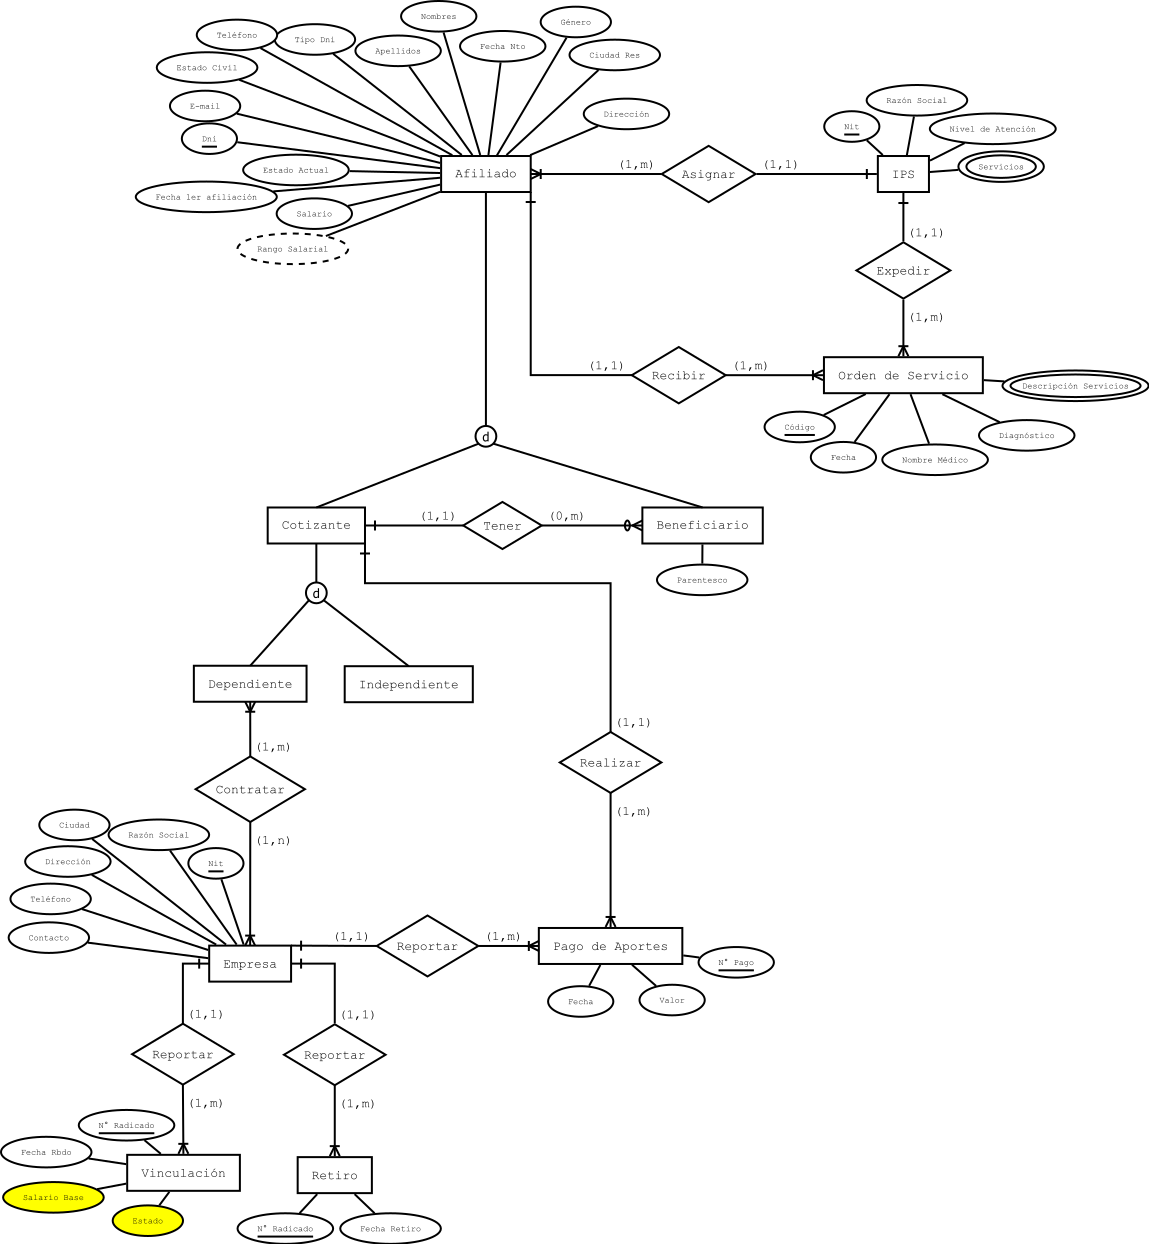
\includegraphics[width=1\textwidth]{Entity_relationship_diagram.pdf} \par}
\caption{Modelo Entidad - Relación.}
\end{figure}
\subsection{Mockups de Interfaz de Usuario}
\begin{figure}[H]
\centering
{\includegraphics[width=1 \textwidth]{Mockup.jpg} \par}
\caption{Mockup de interfaz de login y panel principal.}
\end{figure}
\end{document}